\section{Introduction}
\begin{frame}{Motivation}
	\begin{itemize}
		\item 
		{
			Needing of uncertainty;
			\pause
		} 
		\item 
		{
			Different paths of the future;
		}
	\end{itemize}
\end{frame}
\begin{frame}{Intuition}
	In Computation Tree Logic (CTL) the model of time is a tree-like structure. This way, we cannot use Linear Temporal Logic (LTL) to express the existence of a certain path of time in which some event occurs.
\end{frame}

\begin{frame}{History}
    CTL was defined by:
    
    \begin{columns}[c]
        \begin{column}{.3\textwidth}
            \begin{figure}
                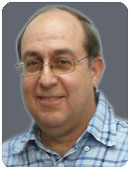
\includegraphics[scale=2]{images/benari.jpg}
                \caption{Mordechai Ben-Ari}
            \end{figure}
        \end{column}
        \begin{column}{.3\textwidth}
            \begin{figure}
                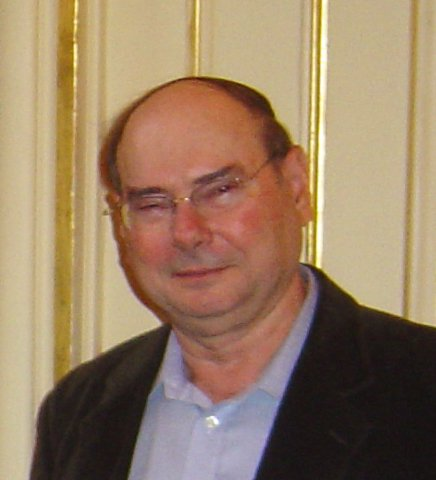
\includegraphics[scale=0.17]{images/Amir_Pnueli.jpg}
                \caption{Amir Pnueli}
            \end{figure}
        \end{column}
        \begin{column}{.3\textwidth}
            \begin{figure}
                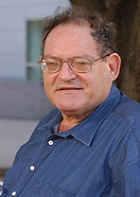
\includegraphics[scale=0.5]{images/manna.jpg}
                \caption{Zohar Manna}
            \end{figure}
        \end{column}
        
    \end{columns}
    
\end{frame}


\begin{frame}{History}
    And, at the same time by:
    
    \begin{columns}[c]
        \begin{column}{.3\textwidth}
            \begin{figure}
                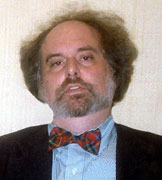
\includegraphics[scale=0.5]{images/E_Allen_Emerson.jpg}
                \caption{Ernest Allen Emerson}
            \end{figure}
        \end{column}
        \begin{column}{.3\textwidth}
            \begin{figure}
                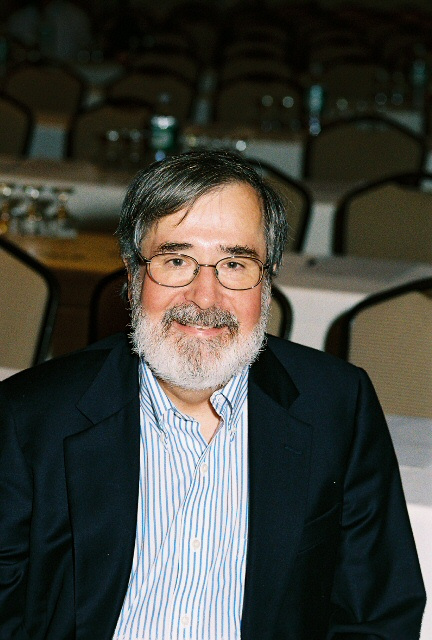
\includegraphics[scale=0.17]{images/Edmund_Clarke.jpg}
                \caption{Edmund Clarke}
            \end{figure}
        \end{column}
    \end{columns}
    
\end{frame}